\chapter{Refactoring}

\section{Code Smells}

\subsection{Code Smell 1: Large Class (God Object)}

Die Klasse \code{PIC} hat zu viele Verantwortlichkeiten (siehe SRP-Analyse). Sie enthält 15+ öffentliche Methoden, verwaltet 8 Felder unterschiedlicher Natur (Hardwarekomponenten, Mutex, Logger, Timing) und ist der zentrale Anlaufpunkt für fast alle Operationen.

\textbf{Lösungsweg:} Die Klasse sollte aufgeteilt werden in:

\begin{itemize}
    \item \code{PICHardware}: hält Register, RAM, Timer (Hardware-Zustand)
    \item \code{PICSimulator}: orchestriert Instruktionsausführung
    \item \code{PICDebugInterface}: bietet thread-sichere Zugriffsmethoden für die UI
\end{itemize}

\begin{lstlisting}[style=codeblock,language=picassocpp]
// Vorher: alles in PIC
class PIC {
    // Hardware-Zustand
    std::shared_ptr<ProgramCounter> pc;
    std::shared_ptr<RAM> ram;
    std::shared_ptr<Timer> timer;

    // Simulationssteuerung
    void getSnapshot(PICSnapshot& snapshot);
    bool tryWriteRegister(uint8_t addr, uint8_t val, std::string* err);
    bool tryToggleBit(uint8_t addr, uint8_t bit, std::string* err);
    bool tryStep(std::string* err);
    // ... 10+ weitere Methoden
};

// Nachher: SRP-Aufteilung
class PICHardware {
    std::shared_ptr<ProgramCounter> pc;
    std::shared_ptr<RAM> ram;
    std::shared_ptr<Timer> timer;
};

class PICSimulator {
    PICHardware& hw;
public:
    bool tryStep(std::string* err);
};

class PICDebugInterface {
    PICHardware& hw;
    PICSimulator& simulator;
    mutable std::mutex executionMutex;
public:
    void getSnapshot(PICSnapshot& snapshot);
    bool tryWriteRegister(uint8_t addr, uint8_t val, std::string* err);
    bool tryToggleBit(uint8_t addr, uint8_t bit, std::string* err);
    bool tryStep(std::string* err);
};
\end{lstlisting}

\subsection{Code Smell 2: Long Method / Switch Statement}

Die Methode \code{Compiler::getInstruction()} enthält eine lange Switch-Kaskade mit etwa 35+ Cases über mehrere Bitmask-Levels.
Dies ist ein typischer \enquote{Long Method}-Smell kombiniert mit einem \enquote{Switch Statement}-Smell.

\textbf{Lösungsweg:} Replace Conditional with Polymorphism / Registry-Pattern:

\begin{lstlisting}[style=codeblock,language=picassocpp]
// Vorher: Lange Switch-Kette in getInstruction()
switch(instruction) {
    case 0x0064: return std::make_unique<CLRWDT>(instruction);
    case 0x0009: return std::make_unique<RETFIE>(instruction);
    // ... ~35 Cases über 4 Switch-Blöcke
}

// Nachher: Factory-Registry
class InstructionRegistry {
    std::vector<std::pair<uint16_t, uint16_t, Factory>> entries;
public:
    void registerInstruction(uint16_t mask, uint16_t pattern, Factory f);
    std::unique_ptr<Instruction> create(uint16_t opcode);
};
\end{lstlisting}

\section{2 Refactorings}

\subsection{Refactoring 1: Extract Class}

\textbf{Bezeichnung:} \emph{Extract Class} – Auslagerung einer in sich geschlossenen
Teilverantwortlichkeit in eine eigene Klasse.

\textbf{Ausgangssituation:}
In \code{terminal_ui.cpp} war die gesamte Rendering-Logik als Nested-Class
\code{TerminalUI::Renderer} direkt in der Translation Unit von \code{TerminalUI}
eingebettet.  Die Nested-Class war über~300 Zeilen lang und mischte
Drawing-Verantwortung mit den übrigen Aufgaben von \code{TerminalUI}.
Das verstößt gegen das Single-Responsibility-Prinzip: Änderungen am Rendering
erforderten Anpassungen in der Hauptdatei der UI-Steuerung.

\begin{figure}[H]
  \centering
  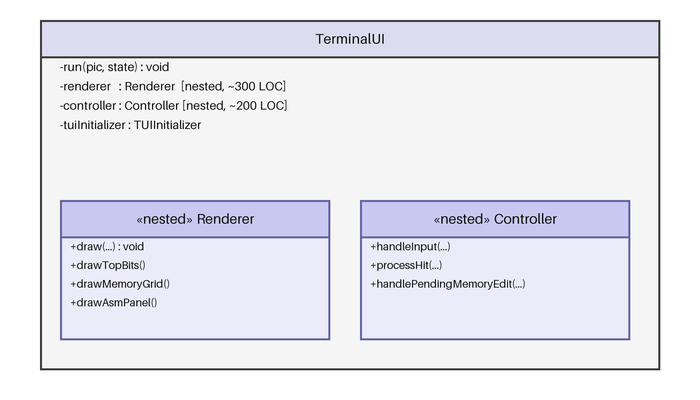
\includegraphics[width=0.55\textwidth]{UML/20.png}
  \caption{UML vor dem Refactoring: \code{Renderer} und \code{Controller} als
           Nested-Classes innerhalb von \code{TerminalUI}.}
\end{figure}

\textbf{Anwendung (Commit \texttt{2f9077e} \enquote{Extracted tui renderer class}):}
Die Nested-Class wurde als eigenständige Klasse \code{TUI_Renderer} in eigene
Dateien (\code{tui_renderer.hpp} / \code{tui_renderer.cpp}) ausgelagert.
\code{TerminalUI} hält seitdem nur noch einen \code{unique_ptr} auf das Objekt
und delegiert alle Zeichenoperationen dorthin.

\begin{lstlisting}[style=codeblock,language=picassocpp]
// Vorher: Renderer-Logik als nested class, definiert in terminal_ui.cpp
class TerminalUI {
private:
    class Renderer; // ~300 Zeilen Rendering-Code in derselben .cpp-Datei
    class Controller;
    std::unique_ptr<Renderer> renderer;
};

// Nachher: eigenstaendige Klasse in tui_renderer.hpp / tui_renderer.cpp
class TUI_Renderer {
public:
    void draw(const PICSnapshot& snapshot,
              SimulationState& state,
              const std::optional<uint8_t>& selectedRamAddress,
              const std::string& loadedPath,
              const std::vector<std::string>& fileLines,
              int manualScrollStart, bool manualScrollEnabled,
              int* renderedStart,
              std::vector<HitBox>& hitBoxes) const;
private:
    static void drawTopBits(...);
    static void drawMemoryGrid(...);
    static void drawAsmPanel(...);
    static void drawControlPanel(...);
};

class TerminalUI {
private:
    std::unique_ptr<TUI_Renderer>     renderer;    // Delegation statt Einbettung
    std::unique_ptr<TUI_Controller>   controller;
    std::unique_ptr<TUIInitializer>   initializer;
};
\end{lstlisting}

\begin{figure}[H]
  \centering
  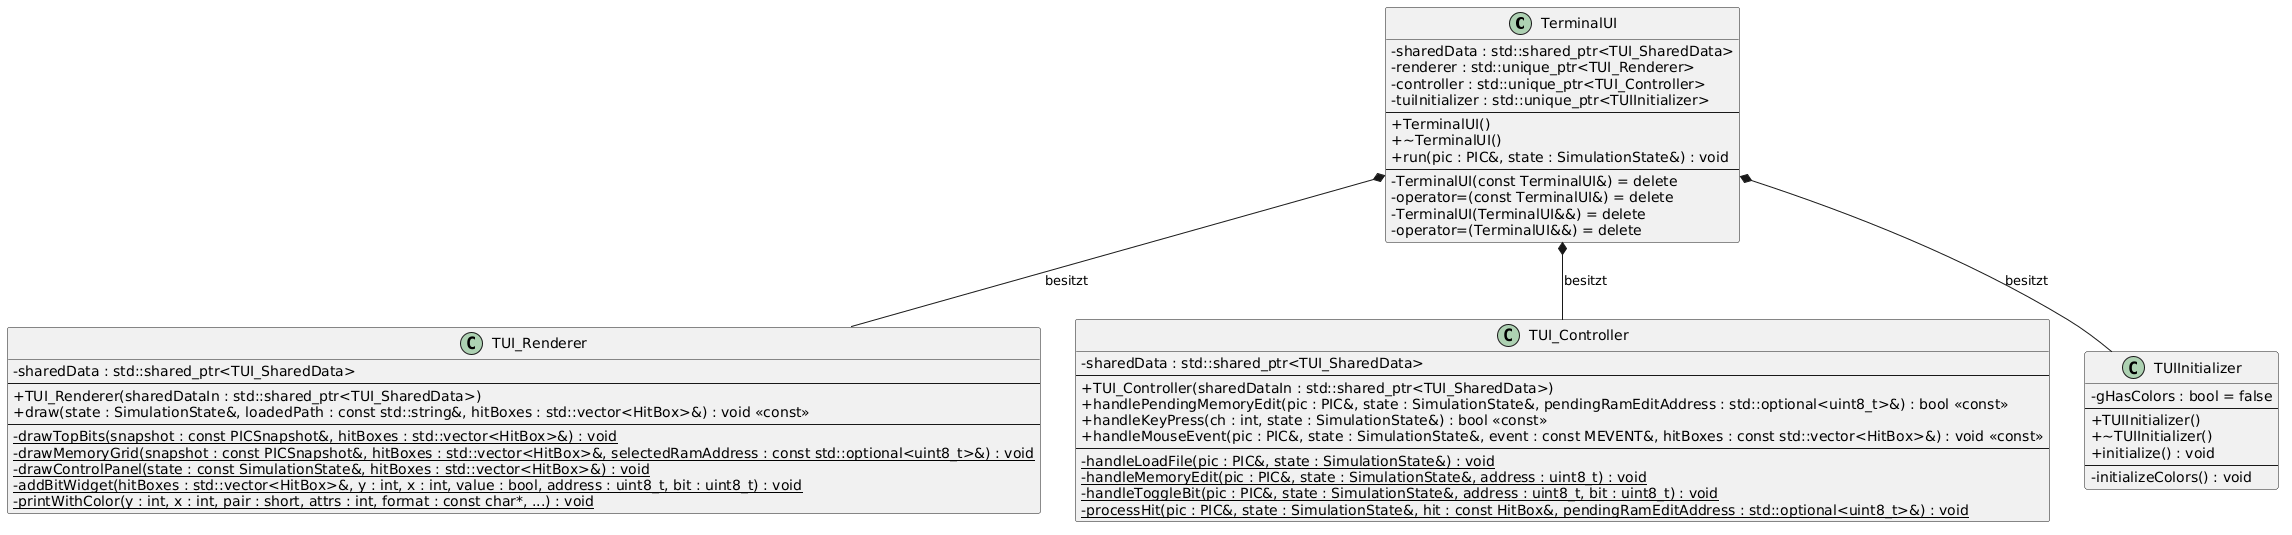
\includegraphics[height=0.3\textwidth,  angle=90]{UML/21.png}
  \caption{UML nach dem Refactoring: \code{TerminalUI} hält Kompositionsbeziehungen
           zu drei eigenständigen Klassen.}
\end{figure}

\textbf{Begründung:}
Durch die Auslagerung besitzt jede Klasse genau eine klar abgegrenzte Aufgabe.
\code{TUI_Renderer} ist unabhängig kompilierbar, separat testbar und kann
ausgetauscht werden, ohne \code{TerminalUI} anzufassen.
Die Kohäsion steigt, die Kopplung sinkt.

% -------------------------------------------------------------------

\subsection{Refactoring 2: Replace Conditional with Polymorphism}

\textbf{Bezeichnung:} \emph{Replace Conditional with Polymorphism} – Ersatz einer
expliziten Typ-Unterscheidung durch virtuellen Dispatch.

\textbf{Ausgangssituation:}
In \code{ALU::executeInstruction()} wurde nach dem Aufruf von \code{execute()}
der konkrete Typ jeder Instruktion über fünf verschachtelte
try-catch-Blöcke zur Laufzeit bestimmt.
Damit war \code{ALU} fest an alle fünf Instruktionskategorien gekoppelt: eine neue
Kategorie hätte einen weiteren Block erfordert und die Methode weiter aufgebläht.

\begin{figure}[H]
  \centering
  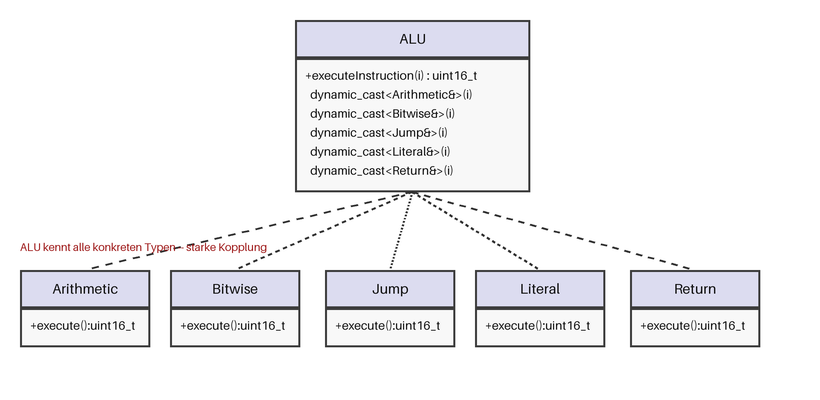
\includegraphics[width=0.82\textwidth]{UML/22.png}
  \caption{UML vor dem Refactoring: \code{ALU} kennt jeden konkreten Instruktionstyp direkt
           (starke Kopplung durch fünf \code{dynamic_cast}-Abhängigkeiten).}
\end{figure}

\textbf{Anwendung (Commit \texttt{170060b} \enquote{Basic run loop}):}
Die gesamte Typunterscheidung wurde entfernt.
Da jede konkrete Instruktionsklasse die rein virtuelle Methode \code{execute()}
der Basisklasse überschreibt, genügt der virtuelle Dispatch – \code{ALU} muss
den konkreten Typ nicht mehr kennen.

\begin{lstlisting}[style=codeblock,language=picassocpp]
// Vorher: Typabfrage per dynamic_cast nach jedem execute()-Aufruf
void ALU::executeInstruction(Instruction& instruction) {
    instruction.execute();
    std::string out = "";
    try { dynamic_cast<Arithmetic&>(instruction); out += "Arithmetic "; }
    catch (const std::bad_cast&) {}
    try { dynamic_cast<Bitwise&>(instruction);    out += "Bitwise ";    }
    catch (const std::bad_cast&) {}
    try { dynamic_cast<Jump&>(instruction);       out += "Jump ";       }
    catch (const std::bad_cast&) {}
    try { dynamic_cast<Literal&>(instruction);    out += "Literal ";    }
    catch (const std::bad_cast&) {}
    try { dynamic_cast<Return&>(instruction);     out += "Return ";     }
    catch (const std::bad_cast&) {}
    if (out == "") out = "NoFit";
    std::cout << out << std::endl;
}

// Nachher: polymorpher Dispatch genuegt vollstaendig
void ALU::executeInstruction(Instruction& instruction) {
    uint16_t executionReturn = instruction.execute();
    return executionReturn;
}
\end{lstlisting}

\begin{figure}[H]
  \centering
  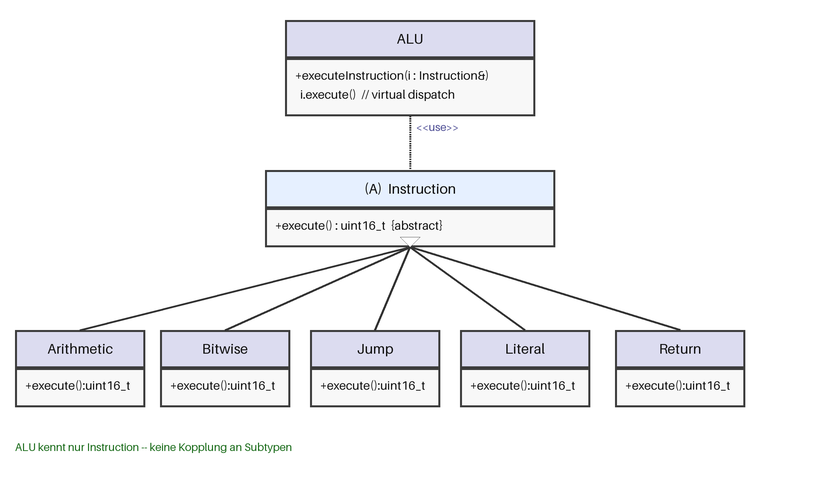
\includegraphics[width=0.72\textwidth]{UML/23.png}
  \caption{UML nach dem Refactoring: \code{ALU} kennt nur die abstrakte Schnittstelle
           \code{Instruction}; konkreter Typ ist zur Kompilierzeit irrelevant.}
\end{figure}

\textbf{Begründung:}
Mit dem virtuellen Dispatch verschwindet jede direkte Abhängigkeit der \code{ALU}
auf konkrete Instruktionsklassen.  Das Offen-Geschlossen-Prinzip wird erfüllt:
neue Instruktionskategorien können hinzugefügt werden, ohne \code{ALU} zu ändern.
Zusätzlich entfällt das ineffiziente Ausnahme-basierte Casting, das bei jedem
Schritt fünf \code{try/catch}-Blöcke durchlief.

